\item \textbf{{[}DHS/PRELIM/9597/2019/P1/Q2{]} }

Dubbed first of its kind globally, the Singapore Quick Response Code
(SGQR) is an infrastructure-light technology that will help to simplify
QR e-payments in Singapore for both consumers and merchants. 

The SGQR is based on the QR Code Specification for Payment System
- Merchant-Presented Mode standard issued by EMVCo, which has the
benefits of international interoperability, multi-tenancy of QR schemes
and non-sensitive data presented for payments. 

According to the specification, the parsed SGQR text string contains
data items, with each data item adhering to the following structure:
id, length, value. Two such data items are highlighted in bold in
the following diagram: 
\begin{center}
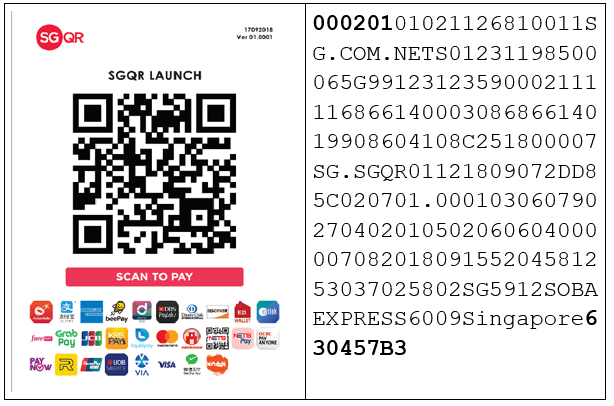
\includegraphics[width=0.5\paperwidth]{C:/Users/Admin/Desktop/Github/question_bank/LyX/static/img/9597-DHS-2019-P1-Q2}
\par\end{center}

Thus for the first data item \texttt{\textbf{000201}}, \texttt{00}
is the id, \texttt{02} is the length, and \texttt{01} is the value. 

And for the last data item \texttt{\textbf{630457B3}}, \texttt{63}
is the id, \texttt{04} is the length, and \texttt{57B3} is the value. 

The value \texttt{57B3} is also a hexdecimal number to verify the
integrity of the SGQR data. 

\subsection*{Task 2.1 }

Write program code to extract the last data item of the SGQR stored
in \texttt{SGQR.TXT}. For the example above, it will be the data item
with id 63 and length 4 i.e. 630457B3. 

\subsection*{Evidence 5 }

Program code. \hfill{} {[}3{]}

\subsection*{Evidence 6 }

Screenshot. \hfill{} {[}1{]}

\subsection*{Task 2.2 }

Write a \texttt{hex2oct} function which takes in a hexadecimal number
string and returns its equivalent octal number string. For example
\texttt{hex2oct('A')} returns \texttt{'12'}. You may not use Python's
built in \texttt{int(num, 8)}, \texttt{int(num, 16)}, \texttt{bin()},
\texttt{oct()} or \texttt{hex()} functions. Use the hexadecimal number
string \texttt{'4F63A'} to to test your program code. 

Hint: One hexadecimal digit can be expressed as four binary digits
and one octal digit can be expressed as three binary digits. 

\subsection*{Evidence 7 }

Program code. \hfill{}{[}5{]}

\subsection*{Evidence 8 }

Screenshot. \hfill{}{[}1{]}

\subsection*{Task 2.3 }

Write program code to perform input validation for a hexadecimal number
string. Test your program with suitable test data. 

\subsection*{Evidence 9 }

Program code. \hfill{}{[}3{]}

\subsection*{Evidence 10 }

Screenshots. \hfill{}{[}2{]}